\chapter{Porovnání účinnosti komprese dat ve formátu XML a JSON}
Poslední kapitola této diplomové práce je zaměřena na aplikaci vybraných kompresních mechanismů na data zapsaná ve formátech XML a JSON. Porovnání bylo provedeno na volně dostupných datech pomocí volně dostupných programů a algoritmů. Naměřené výsledky jsou popsány ve druhé části kapitoly.

\section{Technická parametry testování}

\subsection{Popis zvolených algoritmů}
Pro vzájemné porovnání jsem kromě algoritmů XMill, JSONH a CJSON, které jsou popsány v částech \ref{xmill}, \ref{jsonh} a \ref{cjson}, zvolil i algoritmy LZMA2, BZip2, PPMd, gzip, které nejsou závislé formátu dat. Program XMill byl spouštěn s požadovanými parametry z příkazové řádky, algoritmus CJSON byl spouštěn v prohlížečí Google Chrome verze 42 a mnou implementovaný algoritmus JSONH byl spouštěn jako konzolová aplikace referencující vytvořenou knihovnu. Zbývající 4 algoritmy implementuje program 7-Zip \cite{7zip}, který umožňuje volbu parametrů komprese, jako jsou velikosti slovníku, slova apod.

Algoritmy, které to dovolují, jsem spouštěl s různým nastavením parametrů a k porovnání vybral to nastavení, které produkovalo nejmenší komprimovaný soubor. Velikost těchto parametrů má jistou mez, za kterou už není vliv na velikost komprimovaného souboru tak zásadní. Přitom je ale mezi velikostí parametrů a objemem pamětí potřebné při kompresi přímá úměrnost a takové nastavení nemusí být v případě častého použití efektivní.

\begin{description}
\item[LZMA2] Jde o vylepšenou a optimalizovanou verzi LZ77, která využívá range kodéru a Markovových řetězců (viz \cite{introductionToDataCompression}). Stejně jako LZ77 využívá slovníku, pro který lze uživatelsky zvolit velikost i velikost slova. Proti ostatním algoritmů alokuje při kompresi podstatně více paměti.
\item[BZip2] Algoritmus BZip2 využívá ke kompresi techniky, které nejsou v této práci představeny. Jde o transformace Burrows-Wheelerovu a move-to-front (obě popsány v \cite{introductionToDataCompression}). Tento algoritmus umí pracovat pouze s jedním souborem, což ale pro účely práce nepředstavuje žádný problém.
\item[PPMd] Tato statistická kompresní metoda pracuje s několika modely zároveň. Modely slouží k výpočtu pravděpodobnosti výskytu následujících znaků, které jsou kódovány aritmetickým kódováním (viz \cite{introductionToDataCompression}).
\item[gzip] Tento algoritmus je postaven na programu Deflate, který kombinuje LZ77 a Huffmanovo kódování. Nejprve jsou pomocí LZ77 odstraněny opakující se fráze a poté je výstup ještě zakódován Huffmanovým kódováním. 
\end{description}

\subsection{Popis testovacích souborů}
Testovací data bylo pro účely porovnání bylo nutné získat zapsaná pomocí XML i JSON. Vybraná testovací data jsou volně dostupná ke stažení a to buď přímo ve formátu XML, nebo jako databáze. V prvním případě jsem data transformoval do formátu JSON pomocí frameworku Json.NET \cite{jsonNET}, ve druhém jsem soubory XML i JSON vytvořil. Velikost souborů je volena tak, aby bylo možné provést transformaci, a struktura dat je pro účely testování v každém souboru jedinečná. U popisu jednotlivých souborů uvádím hloubku zanoření, tzn. počet do sebe vnořených elementů pro XML, nebo objektů a polí pro JSON.

\begin{description}
\item[base64img]Soubor 29 obrázků zakódovaných jako řetězec v soustavě o základu 64 popsaných pomocí tří údajů. Hloubka zanoření: 2.\\
Zdroj: %Testovací soubory přiložené k XMill
\item[dblp]
Nehomogenní kolekce bibliografických údajů o periodikách z oblasti počítačových věd. Hloubka zanoření: až 6.\\
Zdroj: %Testovací soubory přiložené k XMill
\item[Employees]
Data z databáze AdventureWorks2008R2 vybraná pomocí příkazu SELECT obsahují 7 převážně textových údajů o 19972 lidech. Hloubka zanoření: 2.\\
Zdroj: %\texttt{msftdbprodsamples.codeplex.com/releases/view/93587}
\item[nasa]
Astronomická data agentury NASA, jde o převážně textová data s údaji o katalozích. Počet elementů 476646, počet atributů: 56317, hloubka zanoření XML: až 8.\\
Zdroj: %\texttt{cs.washington.edu/research/xmldatasets/www/repository.html\#nasa} citováno 27. dubna 2015
\item[SigmodRecord]
Bibliografických údaje o článcích ze stránky sigmod.org. Jsou to převážně textová data -- název článku, jména autorů atd. Hloubka zanoření: 6.\\
Zdroj: %\texttt{dia.uniroma3.it/Araneus/Sigmod/} citováno 27. dubna 2015
\end{description}

\section{Výsledky testování}
Na obrázcích \ref{base64img}, \ref{dblp}, \ref{Employees}, \ref{nasa} a \ref{SigmodRecord} jsou zobrazeny grafy

\begin{figure}[!h]
\centering
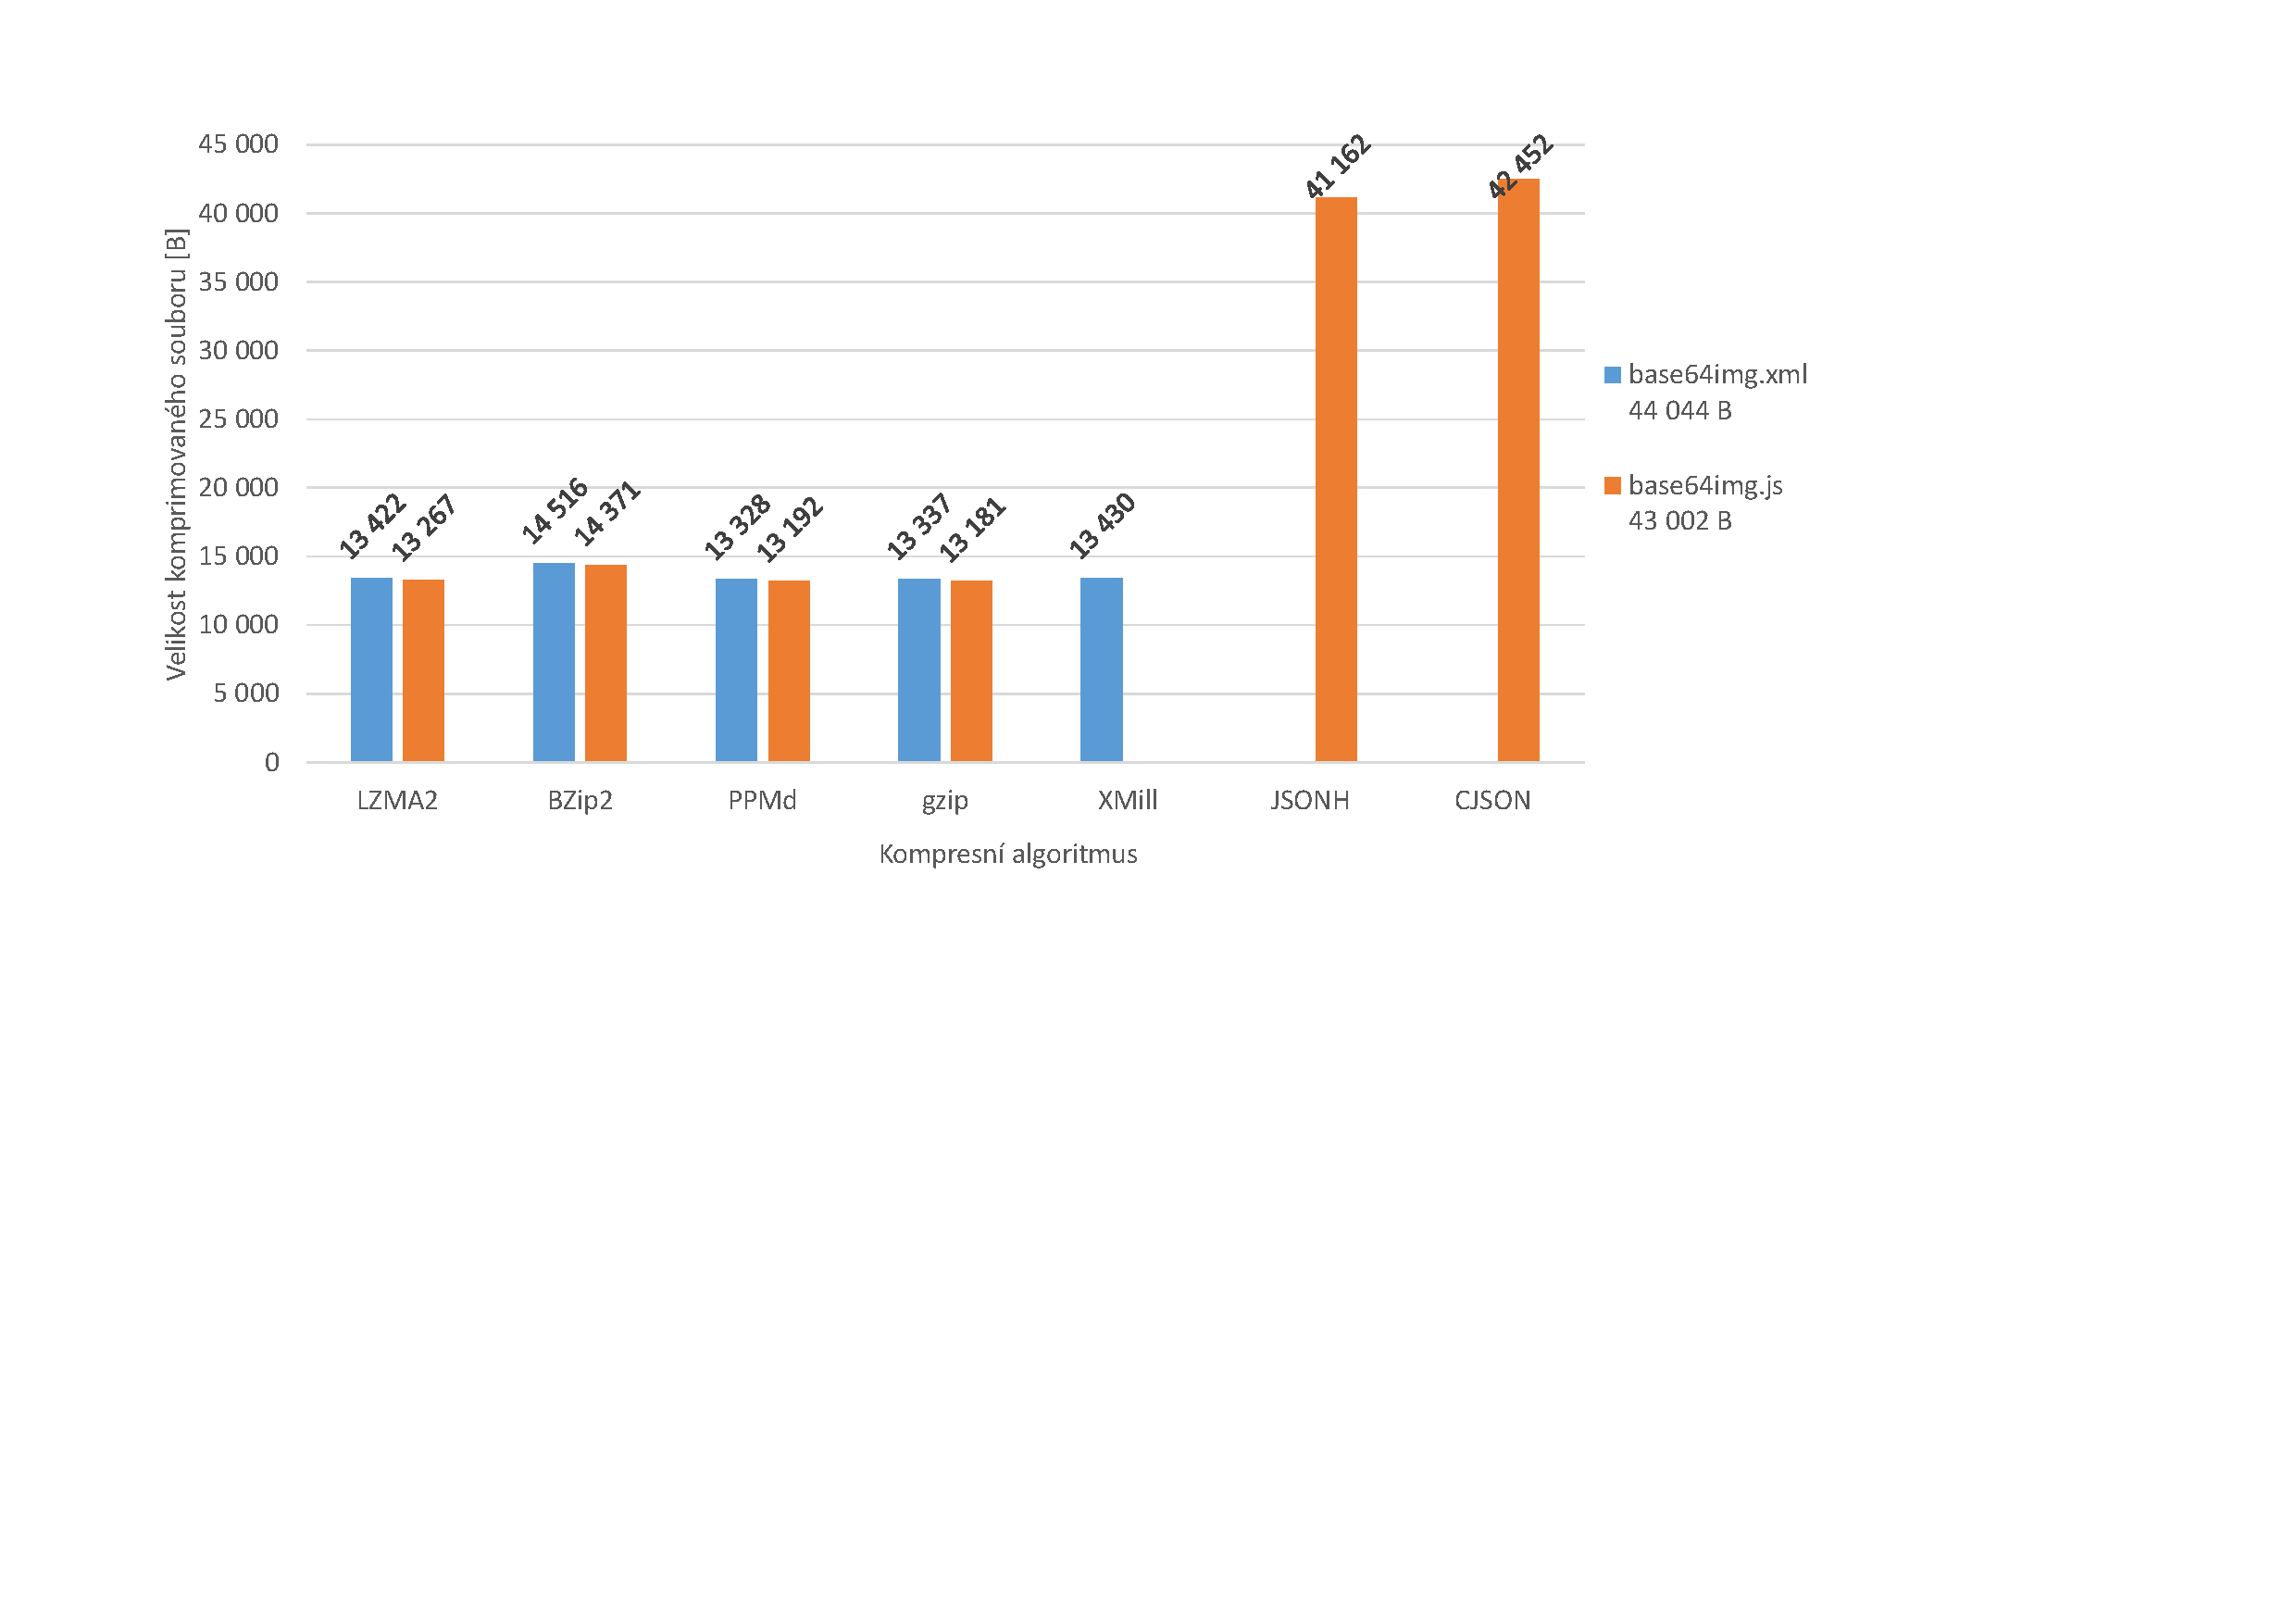
\includegraphics[trim=70 395 200 60, clip, angle=0, width=150mm]{base64img}
\caption{Komprese souborů \texttt{base64img.xml} a \texttt{base64img.js}}
\label{base64img}
\end{figure}

\begin{figure}[!h]
\centering
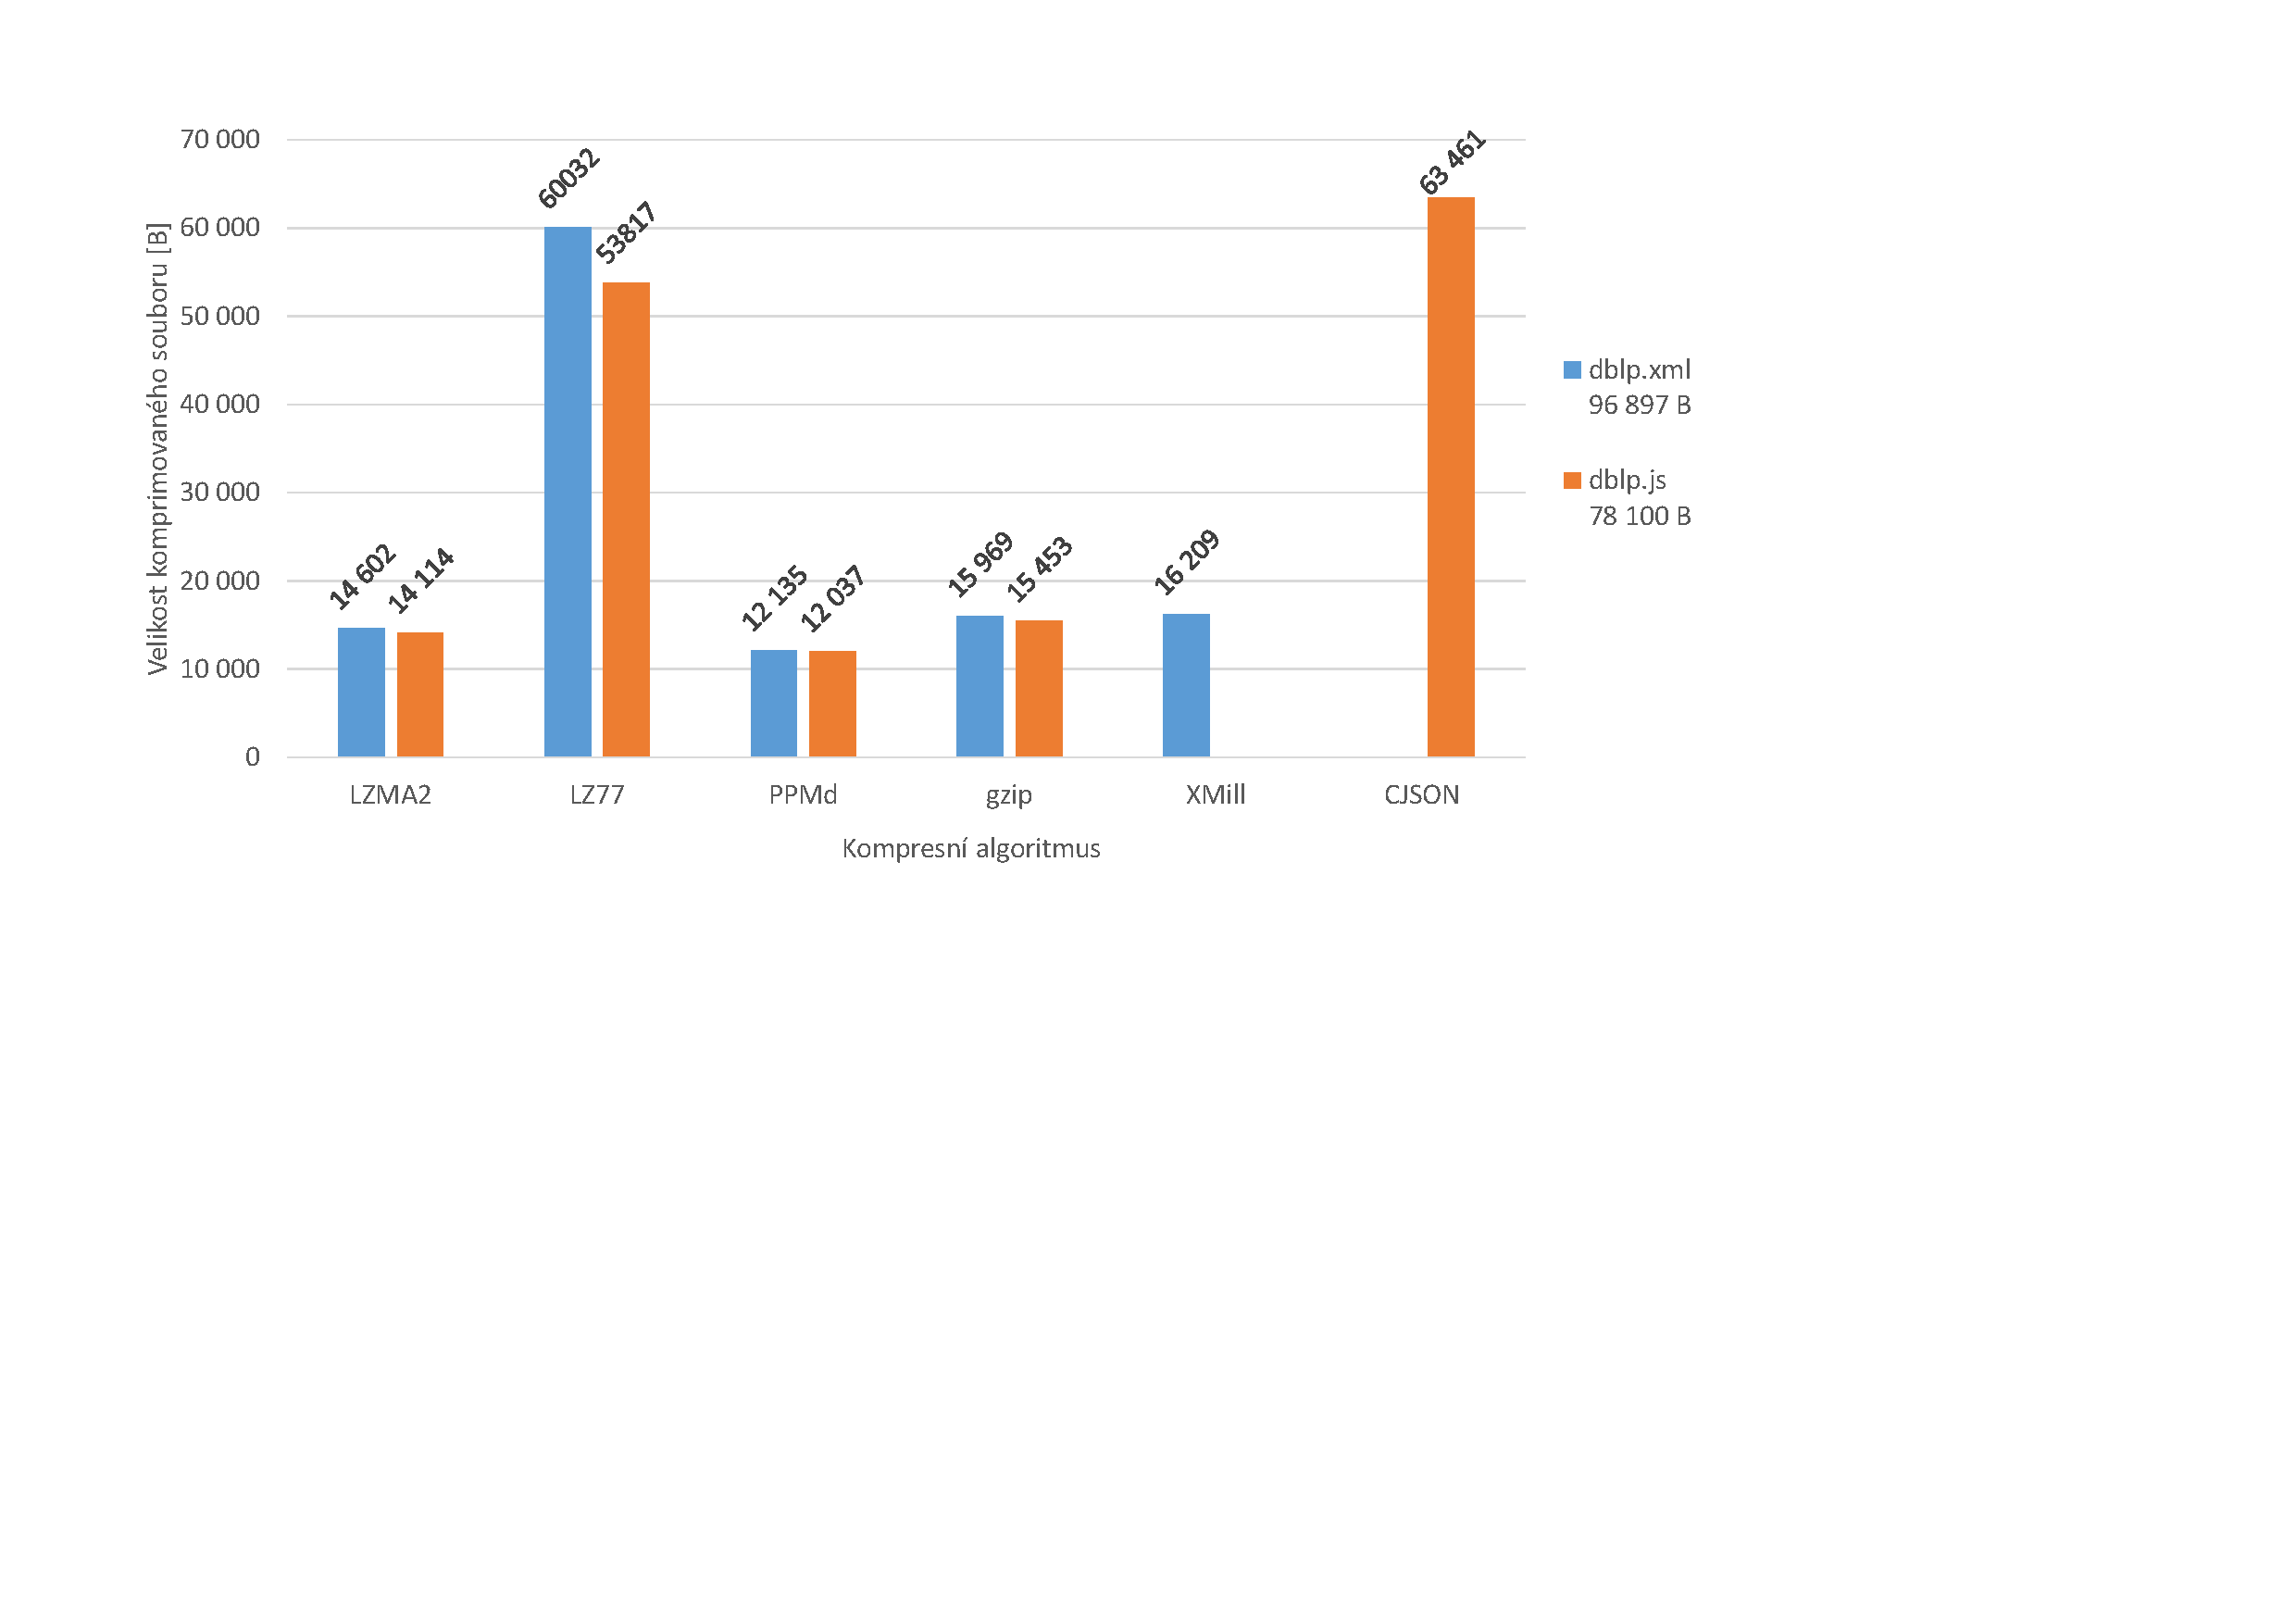
\includegraphics[trim=65 395 260 50, clip, angle=0, width=140mm]{dblp}
\caption{dblp}
\label{dblp}
\end{figure}

\begin{figure}[!h]
\centering
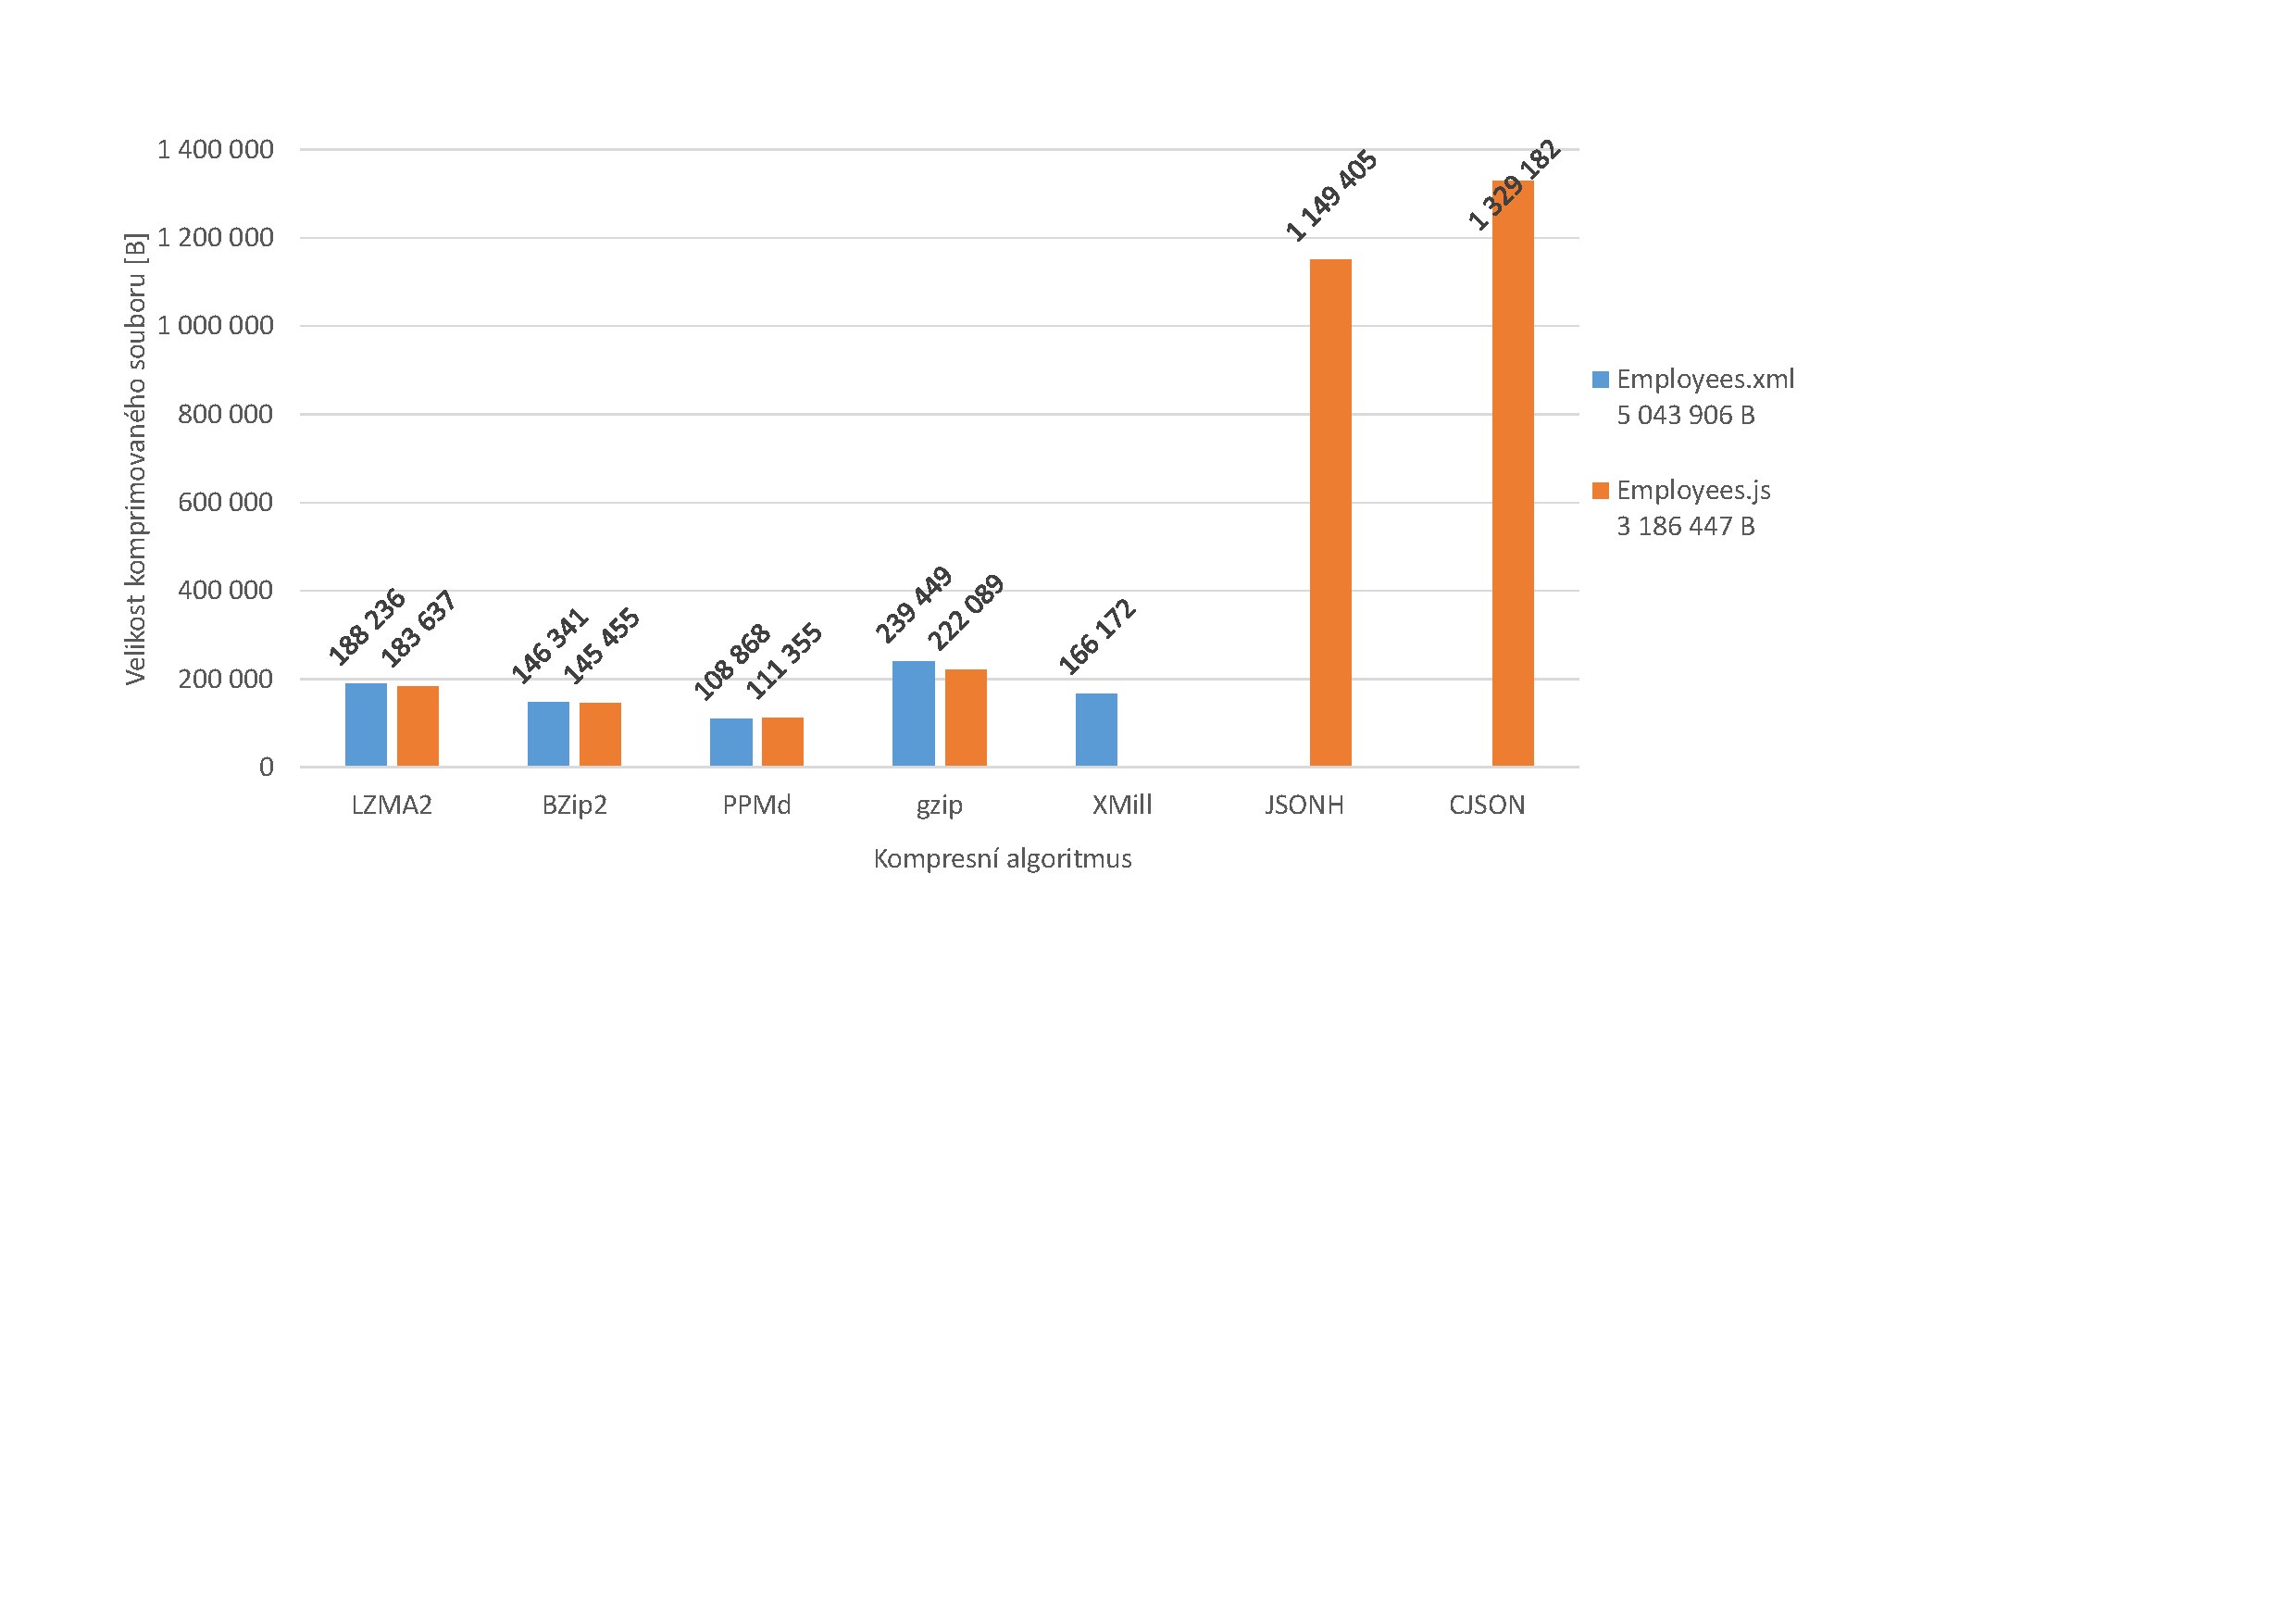
\includegraphics[trim=70 390 200 70, clip, angle=0, width=150mm]{Employees}
\caption{Employees}
\label{Employees}
\end{figure}

\begin{figure}[!h]
\centering
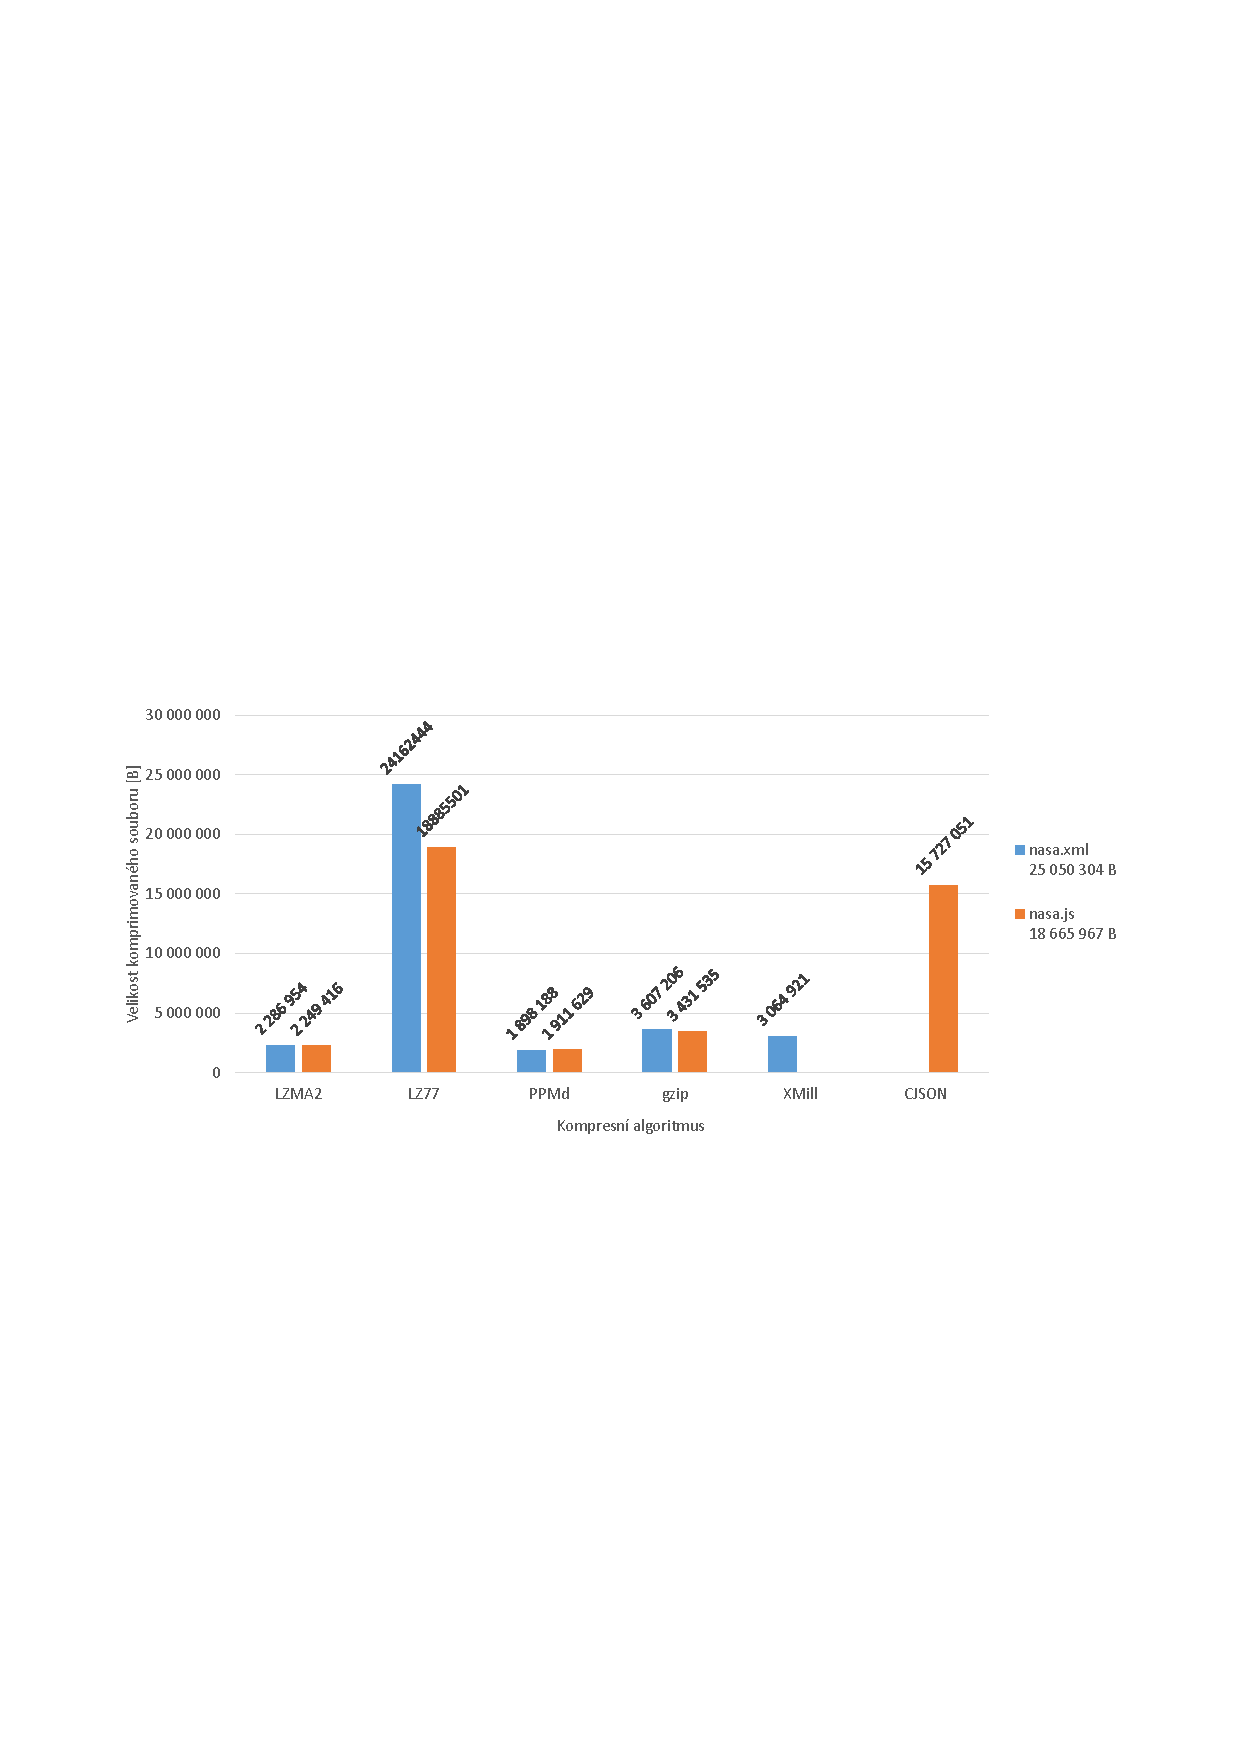
\includegraphics[trim=70 370 200 70, clip, angle=0, width=140mm]{nasa}
\caption{nasa}
\label{nasa}
\end{figure}

\begin{figure}[!h]
\centering
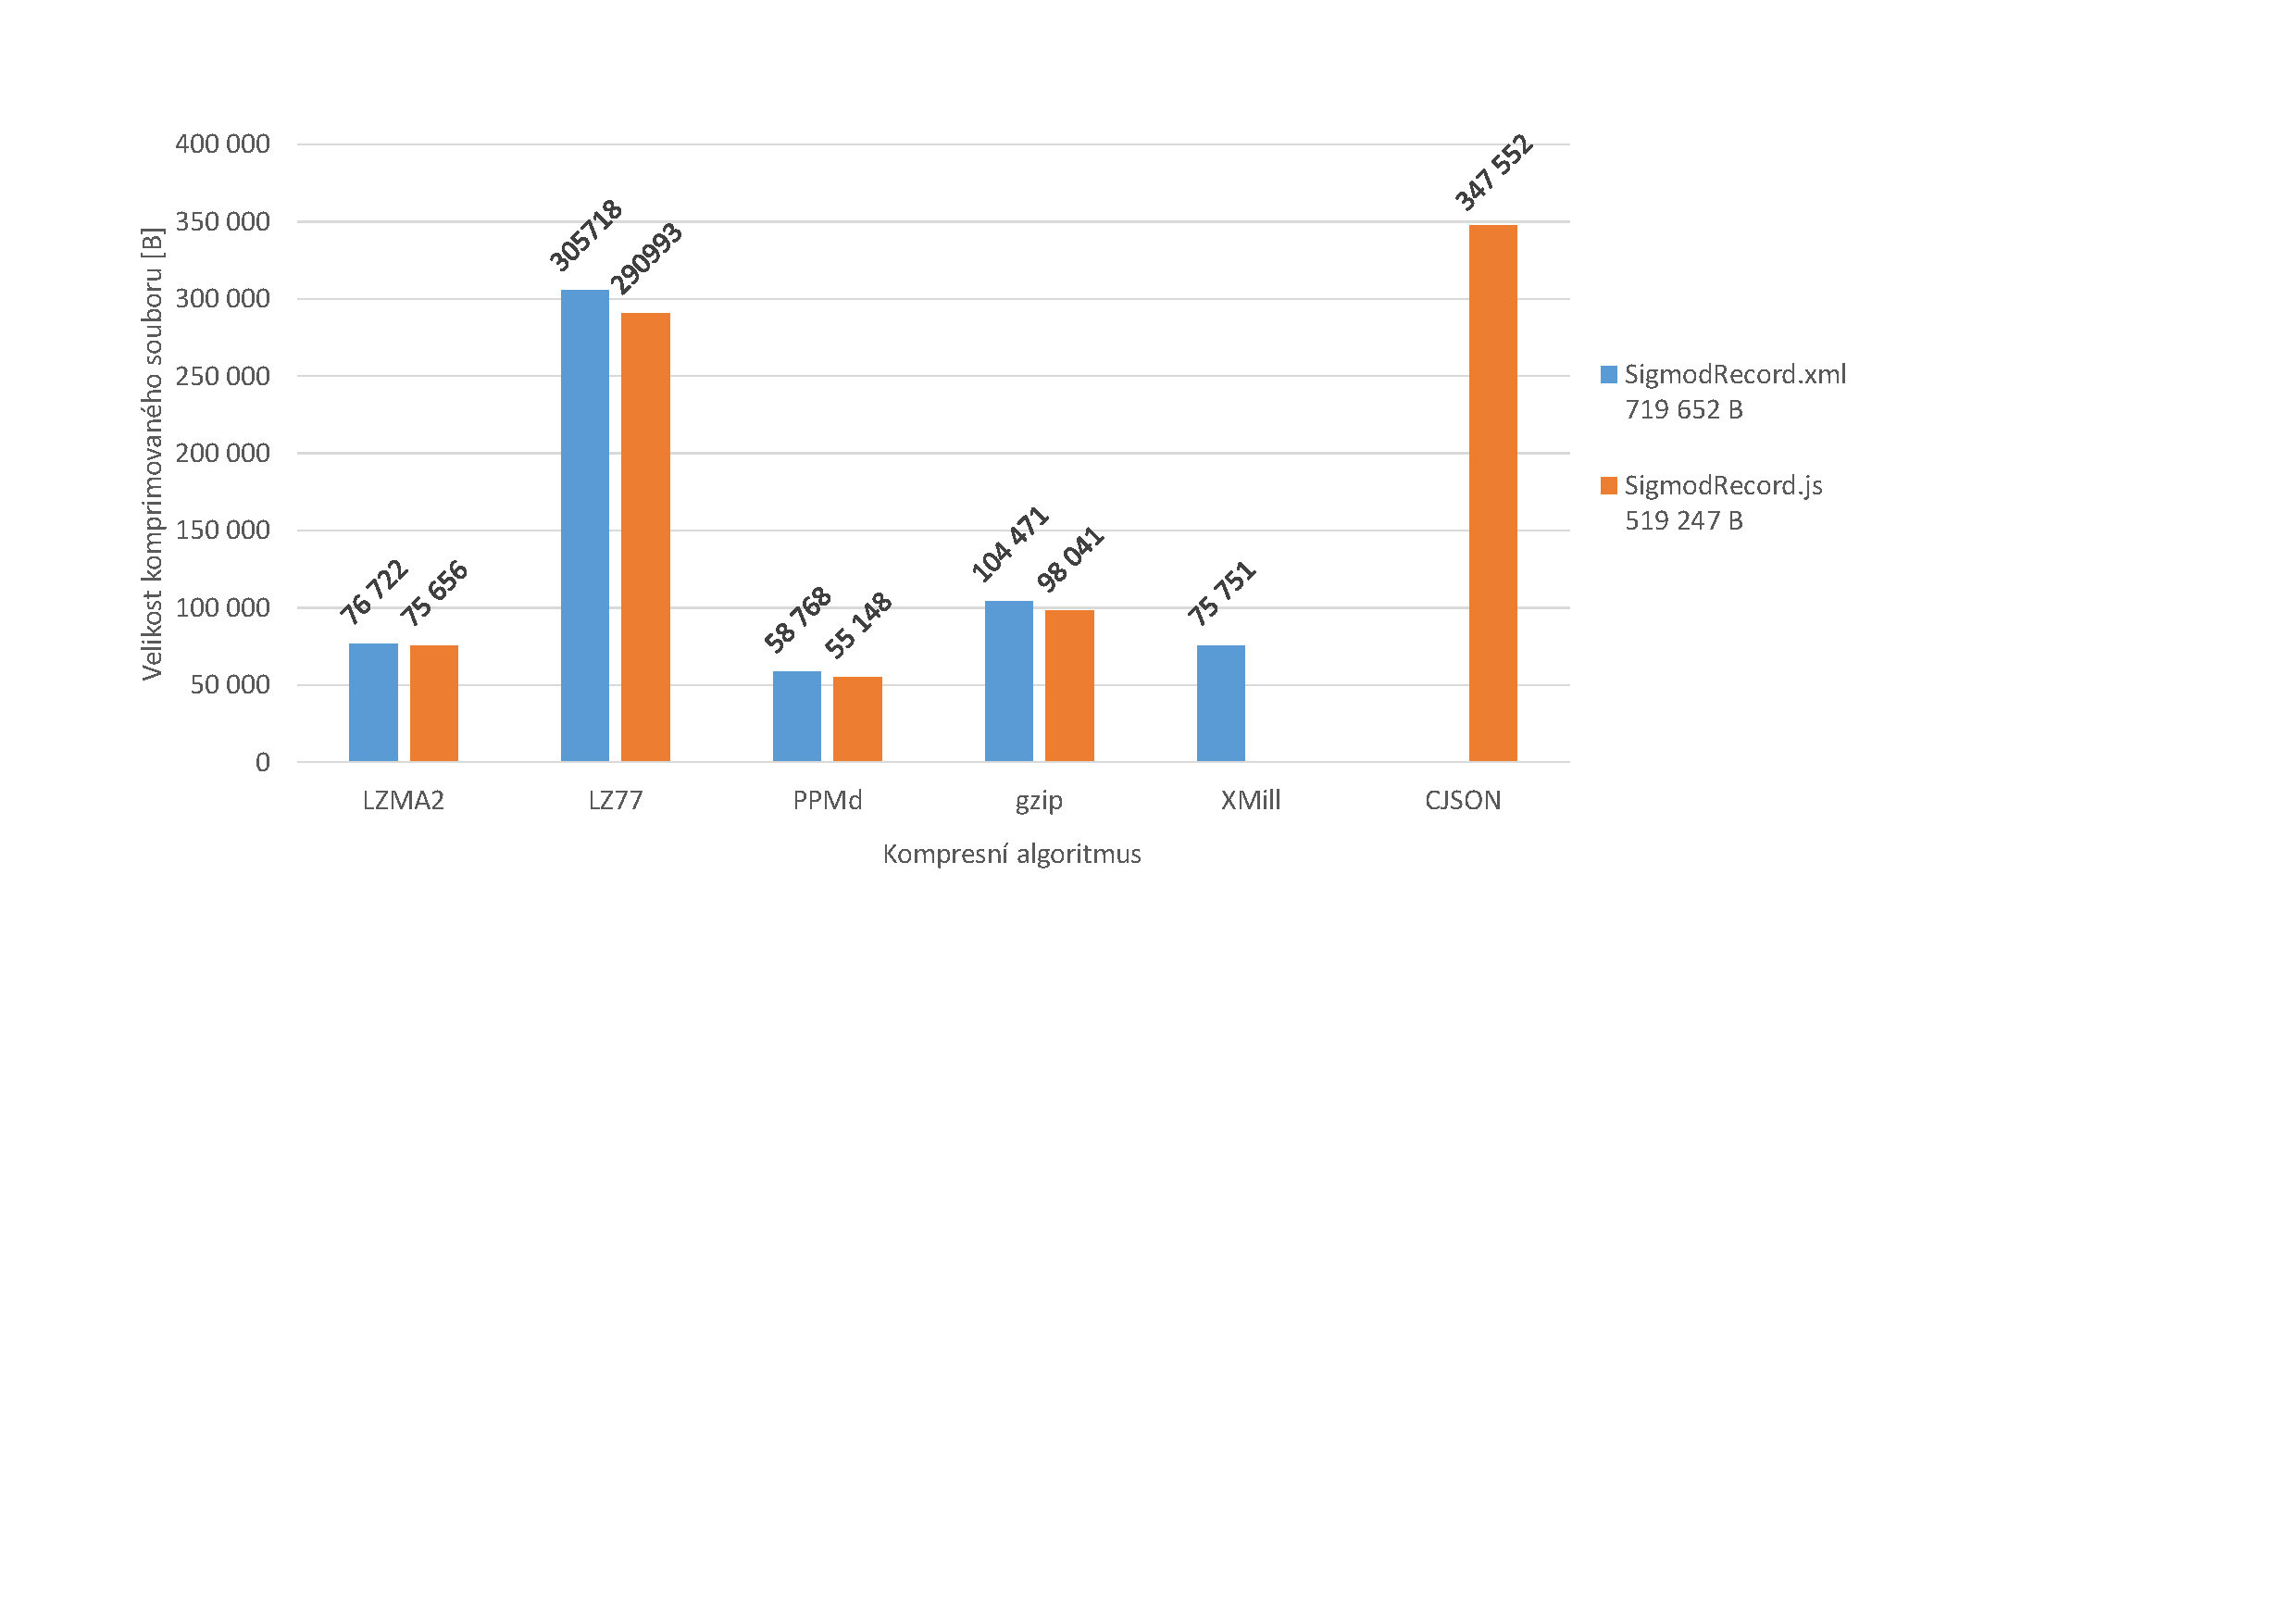
\includegraphics[trim=70 370 200 70, clip, angle=0, width=140mm]{SigmodRecord}
\caption{SigmodRecord}
\label{SigmodRecord}
\end{figure}

\begin{table}[!htb]
\centering
\begin{tabular}{|l|r|r|r|r|r|r|r|}
\hline
 & \multicolumn{7}{|c|}{Kompresní poměr algoritmu}\\
 \cline{2-7}
 Soubor & LZMA2 & BZip2 & PPMd & gzip & XMill & JSONH & CJSON\\
\hline
\end{tabular}
\caption{Kódování textu pomocí algoritmu LZ77}
\label{tabulkaKompresniPomer}
\end{table}